\documentclass{bioinfo}
\copyrightyear{2005}
\pubyear{2005}
\usepackage{amsmath}
\usepackage{afterpage}
\usepackage{algorithm}

%\usepackage{placeins}
\usepackage{algpseudocode}% http://ctan.org/pkg/algorithmicx
\usepackage{xr}
\externaldocument{supplementary_info}
\algnewcommand{\LineComment}[1]{\State \(\triangleright\) #1}

\newcommand{\RR}{I\!\!R} %real numbers
\DeclareMathOperator{\diag}{diag}
\begin{document}
\firstpage{1}

\title[RVD3]{Variant detection model with improved robustness and accuracy for low-depth targeted next-generation sequencing data}
\author[Sample \textit{et~al}]{Corresponding Author\,$^{1,*}$, Co-Author\,$^{2}$ and Co-Author\,$^2$\footnote{to whom correspondence should be addressed}}
\address{$^{1}$Department of XXXXXXX, Address XXXX etc.\\
$^{2}$Department of XXXXXXXX, Address XXXX etc.}

\history{Received on XXXXX; revised on XXXXX; accepted on XXXXX}

\editor{Associate Editor: XXXXXXX}

\maketitle

\begin{abstract}

\section{Motivation:}
Massively parallel sequencing data has been generated by next-generation sequencing (NGS) technology for single nucleotide variants (SNVs) identification among related populations. To address the detection of SNVs, a variety of methods are being under-represented. However, by the reason of the error rate of the clonal heterogeneity and the limitation of the algorithms, identifying the true variants at minor allele frequencies for the very low sequencing read depth remains challenging.

\section{Results:}
We propose a novel empirical Bayesian model to call variants accurately. And the sensitivity of this hierarchical model is analyzed by the improper prior, information prior and non-information prior on the synthetic sequence data with varying read depth and a range of allele frequencies. Our model with information prior (log-normal prior) and non-information prior (Jeffreys prior) both performs a high accuracy (96\%) when applied to a known 0.1\% minor allele frequency within very low read depth (39). Moreover, the model with Jeffreys prior presents much lower false discovery rate (FDR) to a known 0.1\% minor allele frequency event, compared with using improper prior. For further validation, our statistical model was applied on the yeast sequence data which also shows a high specificity and sensitivity over a wide range of read depth. Thus our Bayesian model achieves a enhanced robustness and accuracy when calling variants for the low read depth and minor allele frequencies.
\section{Availability:}


\section{Contact:} \href{name@bio.com}{name@bio.com}
\end{abstract}

\section{Introduction}
Massively parallel sequencing data has been generated by Next-generation sequencing (NGS) technology to benefit clinical diagnostics and sequencing based phylogenetic analyses.
One primary application of NGS is variation detection among related populations and separate novel single-nucleotide variants (SNVs) candidates.
Somatic SNVs are detected by comparing the tumor and corresponding normal samples.

To address the detection of SNVs at low allele frequencies, a number of algorithms from NGS platform are being under-represented.
Strelka \citep{Saunders:2012fh}, VarScan2 \citep{Koboldt:2012cga}, JointSNVMix \citep{roth2012jointsnvmix} are highly used to differentiate somatic SNVs from germline cells.
Also, SAMtools, Genome Analysis Toolkit (GATK) \citep{McKenna:2010bva}, and muTect \citep{Cibulskis:2013ta} broadly concentrate on detecting low-frequency variants.
However identifying the true SNVs remains challenging because of the high false positive rate or high false negative rate which are mainly caused by the clonal heterogeneity.

Recently empirical Bayesian approaches have been made use to identify SNVs.
A empirical Bayesian framework for somatic mutation detection from cancer genome sequencing data - EBCall, enables accurate mutations calling with low allele frequencies (less than 10\%) in a minor tumour subpopulation \citep{shiraishi2013empirical}.
Another method based on empirical Bayesian hierarchical model - RVD, was proposed for ultrasensitive rare SNV detection using beta-binomial model \citep{Flaherty:2011ja}. RVD method is demonstrated to robustly detect mutations at 0.1\% fractional representation, which means accurately call one mutant per every 1000 wild-type alleles.
With the shortcoming of high read depth estimation in RVD, we originally built an improved robustness and accuracy model - RVD3 for low-depth SNVs detection. Variants calling ability is tested and analyzed both on the synthetic sequence data and the true yeast sequencing data with different read depths.

In this article, RVD3 model - a novel Bayesian structure to accurately identify SNVs with small false discovery rate is first described in detail.
Secondly, Metropolis-within-Gibbs sampling is evolved for inference. And then to detect variants, a Bayesian posterior distribution is taken for hypothesis test.
Furthermore, we analyze the sensitivity of the Bayesian model to different priors - Jeffreys prior and log-normal prior, and apply the different priors on the synthetic sequence data.
Finally, we choose Jeffreys prior for the RVD3 model and demonstrate its performance on the yeast sequence data.
The analysis for the results reveals the enhanced robustness and improved accuracy of our algorithm.
%%%%%%%%%%%%%%%%%%
% RVD3 Model
%%%%%%%%%%%%%%%%%%
\section{RVD3 Model}

\subsection{Model Structure}\label{sec:model_structure}
RVD is based on a two-stage hierarchical Bayesian model for variant detection \citep{Flaherty:2011ja}. Through hypothesis test on case and control samples by RVD, we can call the variants successfully. Now RVD3 has three-stage model including priors built on the former RVD model. The definitions for sample data are given: $r_{ji}$ is the number of reads with a non-reference base at position $j$ in replicate $i$, and $n_{ji}$ is the total number of reads at position $j$ in replicate $i$. Three parameters of the model are: $\mu_0$, a global error rate; $M_0$, the global position which estimates the variation in the error rate across the positions; two kinds of priors for $M_j$ are log-normal prior and Jeffreys prior \citep{jeffreys1946invariant}, which enhanced the former RVD model \citep{Flaherty:2011ja}. Here $M_j$ is the local precision measures the alteration in the error rate across replicates at position $j$. The graphical chart for RVD3 is shown in Figure~\ref{fig:graphical_model}.

RVD3 hierarchically includes three levels of samplings: $r_{ji} | n_{ji} \thicksim \text{Binomial}(\theta_{ji}, n_{ji})$ models the variation due to sampling the pool of DNA molecules on the sequencer. $\theta_{ji} \thicksim \text{Beta}(\mu_j, M_j)$ models the variation caused by experimental repeatability. The variation in error rate due to sequence context is modeled by $\mu_j \thicksim \text{Beta}(\mu_0, M_0)$. And the local precision is modeled by $ M_{j} \thicksim \text{log-normal}(\mu, \sigma)$ (log-normal prior), and Jeffreys prior for $M_j$.
%$\pi\left({M}_{j}\right)$

\begin{figure}[h]
\begin{center}
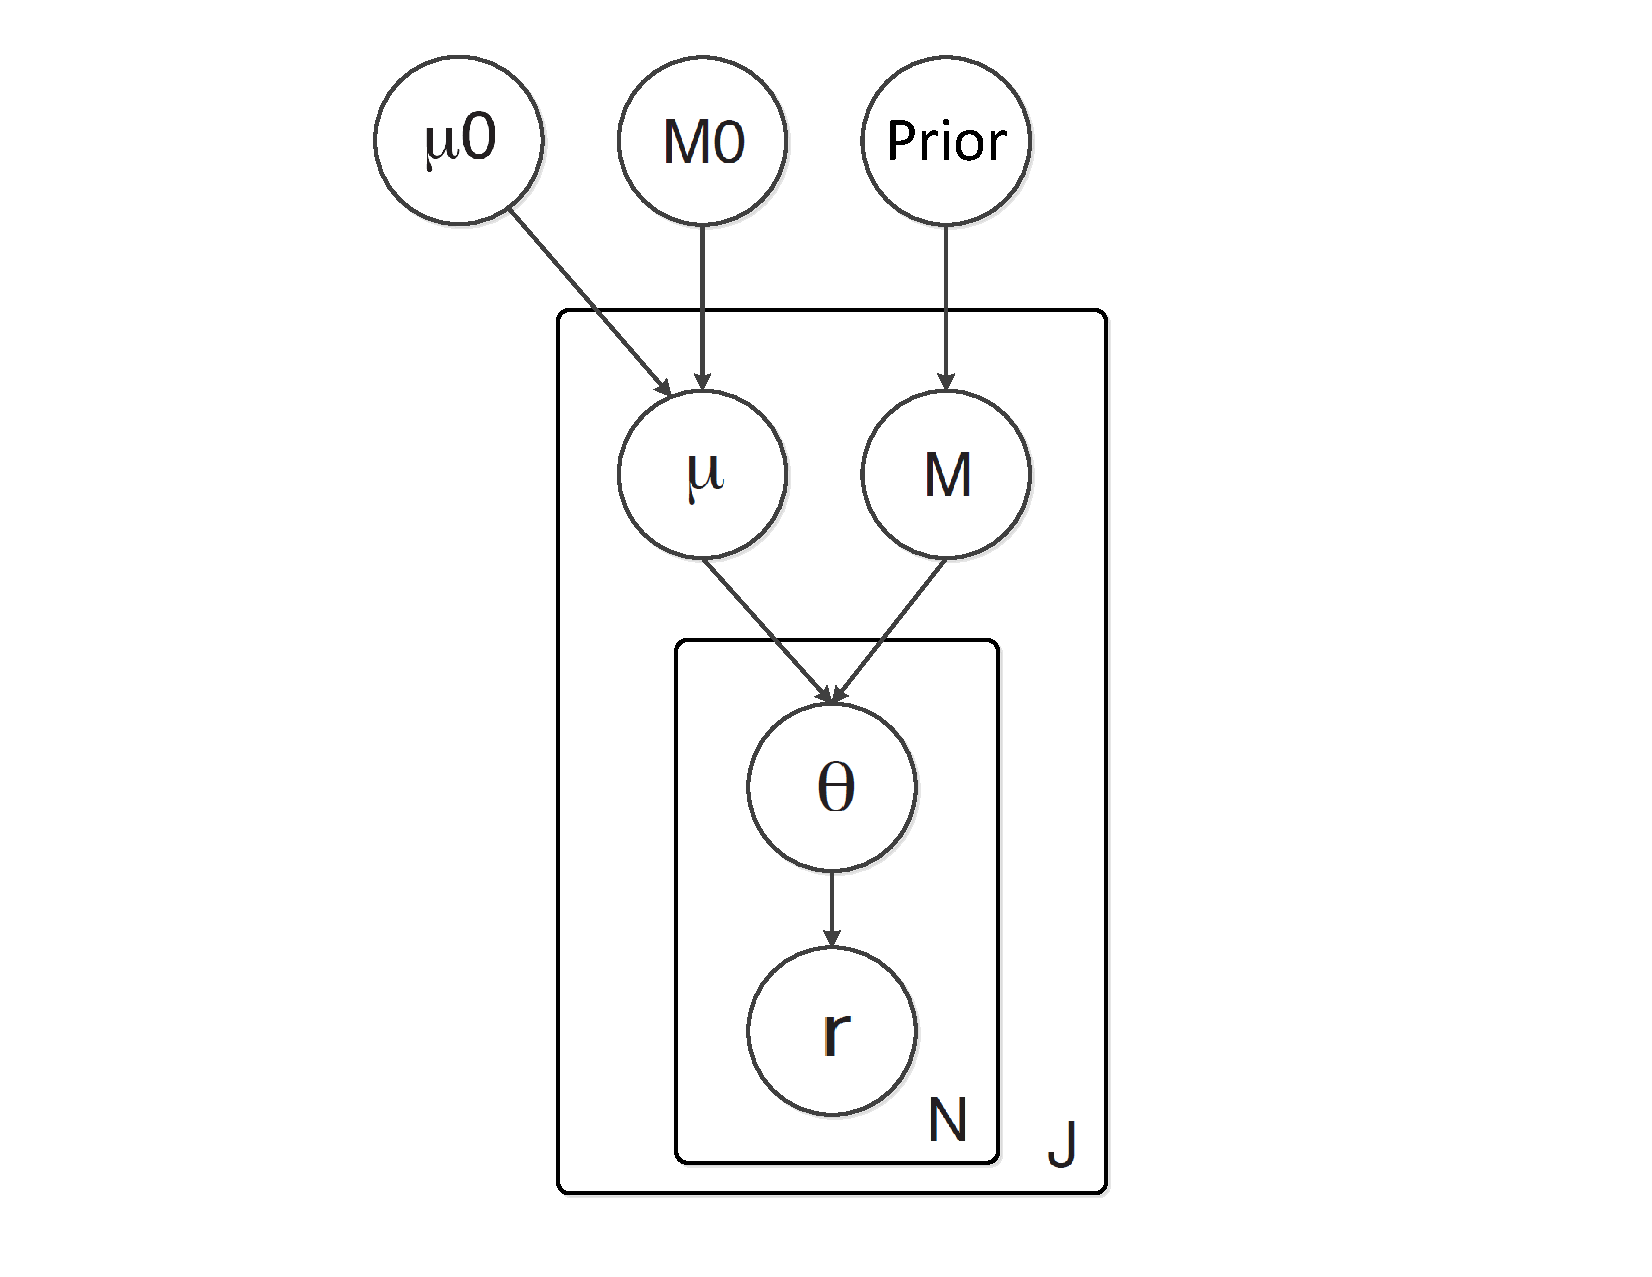
\includegraphics[width=85mm]{figs/RVD3_model.pdf}
\caption{RVD3 Graphical Model}
\label{fig:graphical_model}
\end{center}
\end{figure}


%%%%%%%%%%%%%%%%%%
% Inference & Hypothesis Testing
%%%%%%%%%%%%%%%%%%
\subsection{Inference and Hypothesis Testing}

Metropolis-within-Gibbs sampling is evolved for inference. Algorithm 1 shows the inference process and the detail are also illustrated.

\begin{algorithm}[ht]
\caption{Inference process for Metropolis-within-Gibbs}
\label{alg:metro_gibbs}
\begin{algorithmic}[1]

\State Initialize $\theta$, $\mu$, $M_j$, $\mu_0$, $M_0$
\Repeat
\For {each location j}
  \State Samples from $p \left( \mu_j |\theta_{ij},\mu_0,M_0\right)$ \Comment{Sample $\mu_j$}
  \State Set $\mu_j$ to the sample median for the samples
  \State Samples from $p \left( M_{j} |\mu,\sigma, \theta_{ji},\mu_j\right)$ \Comment{Sample $M_j$}

  \For {each replicate i}
	\State Sample from $p \left( \theta_{ij} |r_{ij},n_{ij},\mu_j,M \right)$ \Comment{Sample $\theta_{ji}$}
  \EndFor

\EndFor
\Until {sample size sufficient}
\end{algorithmic}
\end{algorithm}

%%%%%%%%%%%%%
% Initialization
%%%%%%%%%%%%%
\subsubsection{Initialization}
The initial values for the model parameters and latent variables is obtained by a method-of-moments (MoM) procedure. MoM works by setting the population moment equal to the sample moment. A system of equations is formed such that the number of moment equations is equal to the number of unknown parameters and the equations are solved simultaneously to give the parameter estimates. We simply start with the data matrices $r$ and $n$ and work up the hierarchy of the graphical model solving for the parameters of each conditional distribution in turn.

The initial parameter estimates and derivations are provided in Appendix~\ref{sec:appendix_mom}. Below is the MoM estimate for replicate-level parameters
$\tilde{\theta}_{ji} = \frac{r_{ji}} {n_{ji}}$.
The estimates for the position-level parameters are
$\tilde{\mu}_j = \frac{1}{N} \sum_{i=1}^N \theta_{ji}$
and
$\tilde{M_j} = \frac{ \tilde{\mu}_j (1 - \tilde{\mu}_j ) } { \frac{1}{N} \sum_{i=1}^N \theta_{ji}^2 } -1$.
The estimates for the genome-level parameters are
$\tilde{\mu}_0 = \frac{1}{J} \sum_{j=1}^J \mu_j$
and
$\tilde{M}_0 = \frac{ \tilde{\mu}_0 (1 - \tilde{\mu}_0 ) } {\frac{1}{J} \sum_{j=1}^J \mu_j^2 } -1$.

%%%%%%%%%%%%%%%%%%
% Sampling theta
%%%%%%%%%%%%%%%%%%
\subsubsection{Sampling from $p \left( \theta_{ij} |r_{ij},n_{ij},\mu_j,M \right)$}

Because the Bayesian conjugacy between the prior
$p(\theta_{ji} | \mu_j, M_j) \thicksim \text{Beta}(\mu_j, M_j)$
and the likelihood
$p(r_{ji} | n_{ji}, \theta_{ji}) \thicksim \text{Binomial}(\theta_{ji}, n_{ji})$,
we draw the samples from the posterior distribution
$p(\theta_{ji} | r_{ji}, n_{ji}, \mu_j, M_j)$
The posterior distribution is
\begin{equation}
	p(\theta_{ji} | r_{ji}, n_{ji}, \mu_j, M_j) \thicksim \text{Beta}\left( \frac{r_{ji} + M_j \mu_j}{n_{ji} + M_j} , n_{ji} + M_j\right).
\end{equation}

%%%%%%%%%%%%%%%%%%
% Sampling mu
%%%%%%%%%%%%%%%%%%
\subsubsection{Sampling from $p \left( \mu_j |\theta_{ji},M_j,\mu_0,M_0\right)$}
Based on Markov blanket, the posterior distribution over $\mu_j$ is
\begin{equation}
	p( \mu_j | \theta_{ji}, M_j, \mu_0, M_0 ) \propto p(\mu_j | \mu_0, M_0) p(\theta_{ji} | \mu_j, M_j).
\end{equation}

Since the prior, $p(\mu_j | \mu_0, M_0)$, is not conjugate to the likelihood, $p(\theta_{ji} | \mu_j, M_j)$, we sample from the posterior distribution using the Metropolis-Hastings algorithm. By experience when $\mu_j^{(p)} \in (10^{-3},1-10^{-3})$, the proposal distribution variance for all the Metropolis-Hastings steps within a Gibbs iteration is set to $\sigma_j = 0.1 \cdot \mu_j^{(p)}$ ; otherwise, we set $\sigma_j = 10^{-4}$ if $\mu_j^{(p)}< 10^{-3}$ and $\sigma_j = 10^{-1}-10^{-4}$ if $\mu_j^{(p)}>1-10^{-3}$. We have found that the algorithm performance improves when we take the median of five or more M-H samples as a single Gibbs step for each position.

(Copy) We resampled from the proposal if the sample is outside of the support of the posterior distribution. We typically discard 20\% of the sample for burn-in and thin the chain by a factor of 2 to reduce autocorrelation among samples. Since, each position $j$ is exchangeable given the global hyperparameters $\mu_0$ and $M_0$ this sampling step can be distributed across up to $J$ processors.

%%%%%%%%%%%%%%%%%%
% Sampling Mj
%%%%%%%%%%%%%%%%%%
\subsubsection{Sampling from $p \left( M_{j} |\mu,\sigma, \theta_{ji},\mu_j\right)$}
Since Jeffreys prior is from the Fisher information and in RVD3 model ${\theta }_{ji}\sim Beta\left( {\mu }_{j},{M}_{j}\right)$,

\begin{equation}\label{equ:JefferyInference}
I\left({M}_{j}\right)={E}_{{M}_{j}}\left[ -\frac{\delta ^{2}\log p\left(\theta _{j}|\mu_{j},M_{j}\right)}{\delta M^{2}_{j}}\right]
\end{equation}

We calculated the equations Appendix~\ref{sec:appendix_Jeffreys} and obtained the Jeffreys' prior for $M_j$:

% \pi\left({M}_{j}\right) =
\begin{equation}
[-\left(\Psi_{1}(M_{j}) - \Psi_{1}(\mu_{j} M_{j})\mu_{j}^{2} - \Psi_{1}((1-\mu_{j})M_{j}){(1-\mu_{j})^{2}}\right)]^{\frac{1}{2}}
\end{equation}

For log-normal prior, the posterior distribution over $M_{j}$ given its Markov blanket is

\begin{equation}
	p( M_{j} |\mu, \sigma, \theta_{ji},\mu_j) \propto p(\theta_{ji} | \mu_j, M_j) p(M_{j} | \mu, \sigma)
\end{equation}

We have $ \theta_{ji}\thicksim\text{Beta}(\mu_{j},M_{j})$, and $ M_{j} \thicksim \text{log-normal}(\mu, \sigma)$. Since we cannot provide an interpretive form for it, Metropolis-Hastings algorithm was still used to sample from the posterior distribution.


%%%%%%%%%%%%%%%%%%
% Posterior Density Test
%%%%%%%%%%%%%%%%%%
\subsubsection{Posterior Density Test}\label{sec:hypothesis_test}
Posterior distributions of $\mu_j$ for the control and case are achieved -  $\tilde{\mu}_j^{\text{case}}$ and $\tilde{\mu}_j^{\text{control}}$, by Metropolis-within-Gibbs. So we called a variant when $\tilde{\mu}_j^{\text{case}} > \tilde{\mu}_j^{\text{control}}$ with $1-\alpha$ confidence,
\begin{equation}\label{eqn:bayes_test}
	\Pr( \tilde{\mu}_j^{\text{case}} - \tilde{\mu}_j^{\text{control}} \geq \tau ) > 1-\alpha,
\end{equation}
where $\tau$ is a detection threshold and $1-\alpha$ is the confidence level. We set $\tau = 0$ in our experiment [XXX].


%%%%%%%%%%%%%%%%%%
% Chi^2 Test
%%%%%%%%%%%%%%%%%%
\subsubsection{$\chi^2$ test for non-uniform base distribution}
($\chi^2$ test is totally Copied!)
An abundance of non-reference bases at a position called by the posterior density test may be due to a true mutation or due to a random sequencing error; we would like to differentiate these two scenarios. We assume non-reference read counts caused by a non-biological mechanism results in a uniform distribution over three non-reference bases. In contrast, the distribution of counts among three non-reference bases caused by biological mutation would not be uniform.

We use a $\chi^2$ goodness-of-fit test on a multinomial distribution over the non-reference bases to distinguish these two possible scenarios. The null hypothesis is $H_0: p = (p_1, p_2, p_3)$ where $p_1=p_2=p_3=1/3$. Cressie and Read (1984) identified a power-divergence family of statistics, indexed by $\lambda$, that includes as special cases Pearson's $\chi^2 (\lambda = 1)$ statistic, the log likelihood ratio statistic $(\lambda = 0)$, the Freeman-Tukey statistic $(\lambda = -1/2)$, and the Neyman modified statistic $X^2 (\lambda = -2)$. The test statistic is

\begin{equation}
 2nI^\lambda = \frac{2}{\lambda(\lambda+1)}\sum_{k=1}^3 r_{ji}^{(k)} \left[\left(\frac{r_{ji}^{(k)}}{E_{ji}^{(k)}}\right)^\lambda-1\right];\lambda \in R,
\end{equation}

where $r_{ji}^{(k)}$ is the observed frequency for non-reference base $k$ at position $j$ in replicate $i$ and $E_{ji}^{(k)}$ is the corresponding expected frequency under the null hypothesis. \citet{cressie1984multinomial} recommended $\lambda = 2/3$ when no knowledge of the alternative distribution is available and we choose that value.

We control for multiple hypothesis testing in two ways. We use Fisher's combined probability test \citep{fisher1970statistical} to combine the p-values for $N$ replicates into a single p-value at position $j$,

\begin{equation}\label{eqn:fisher_combined}
	X_j^2 = -2 \sum_{i=1}^N \ln(p_{ji}).
\end{equation}

Equation~\eqref{eqn:fisher_combined} gives a test statistic that follows a $\chi^2$ distribution with $2N$ degrees of freedom when the null hypothesis is true. Finally, we use the Bejamini-Hochberg method to control the family-wise error rate (FWER) over positions that have been called by the Bayesian hypothesis test~\eqref{eqn:bayes_test} \citep{benjamini1995controlling, efron2010large}.

%%%%%%%%%%%%%%%%%%%%%%%%
% Priors for precision parameter
%%%%%%%%%%%%%%%%%%%%%%%%
\subsection{Priors for precision parameter}
%\subsubsection{Improper Prior}
The prior distribution characterizes the knowledge of the parameters in the model. Including prior information in the Bayesian approach is difficult but meaningful. An improper prior is the prior distribution integrates to infinity, and may cause an improper posterior which results in an invalid inferences \citep{lesaffre2012bayesian}. Furthermore when the Markov chain Monte Carlo method is taken to derive the posterior, it is possibly hard to sniff out the improper posterior. Even though no problems happened in estimation by improper prior, other troubles could be caused in the Bayesian inference and analysis by it \citep{stein1965approximation}. Playing no prior on $ M_{j}$ is exactly an implicit improper prior. Therefore we considered about non-information prior and information prior.

%\subsubsection{Jeffreys Prior}
Various noninformative prior distributions have been suggested for parameters in hierarchical models. Jeffreys prior, as a typical and influential one, is proposed to establish a least informative prior that is automatically invariant to transformations by Harold Jeffreys \citep{jeffreys1946invariant}. It is defined in terms of the Fisher information and works well with a single parameter. In our research Jeffreys prior for $M_j$ is the square root of Fisher information of $M_j$.

A good informative prior is imperative to promote accurate posterior estimates. In our study, log-normal prior is a typical prior for the beta density's parameters, $\theta_{ji} \thicksim \text{Beta}(\mu_j, M_j)$. The parameters of it denoted $\mu$ (mean) and $\sigma$ (standard deviation) respectively.

%%%%%%%%%%%%%%%%%%
% Data Sets
%%%%%%%%%%%%%%%%%%
\section{Data Sets}

\subsection{Synthetic DNA Sequence Data}

Two 400bp DNA sequences differ only 14 single nucleotide positions. Sample of the case and control DNA were mixed to yield 0.1\%, 0.3\%, 1\%, 10\%, and 100\% defined minor allele frequencies (MAFs). The details of the experimental protocol are available from the original publication~\citep{Flaherty:2011ja}. We used BWA v0.7.5a to align the reads to the reference sequence with the -C50 option to remove the reads of high mapping quality. BAM files were sampled by $10\times$, $100\times$, $1,000\times$, and $10,000\times$ using Picard v1.104 (http://picard.sourceforge.net). The final data set contains read pairs for $N=6$ replicates for the control at different MAF levels.

\subsection{Yeast Data}
We first mapped the wild-tpye strain GSY1135 \citep{kvitek2011reciprocal} to Chromosome 10 in S288c reference genome (SGD; http://www.yeastgenome.org/) by BWA v0.7.5a \citep{li2009fast}. Then called SNPs by GATK v2.5 UnifiedGenotyper \citep{McKenna:2010bva, depristo2011framework} and created a FASTA GSY1135 reference using GATK FastaAlternative.
Secondly, we downloaded generation 7 as control and generation 133 as case in experiment 1 from \citep{kvitek2013whole}, and removed WT population using FASTX Barcode Splitter and trimed the Nextera tag by Cutadapt v1.3.
Finally, the FASTQ files of case and control were mapped to the corresponding reference genome created before. And pileup files were generated using Samtools v0.1.19 and depth chart file were derived by randomly down sampling.


%%%%%%%%%%%%%%%%%%
% Results
%%%%%%%%%%%%%%%%%%
\section{Results}

%%%%%%%%%%%%%%%%%%
% Sensitivity analysis of priors
%%%%%%%%%%%%%%%%%%
\subsection{Sensitivity analysis of priors}
In order to examine the robustness of RVD3 to changes of different priors, we performed information prior (log-normal) and non-information prior (Jeffreys). We found that RVD3 is robust to changing the priors. The RVD3 algorithm provides estimates of model parameters and latent variables given the data.

We show several of these parameters of the model with Jeffreys prior in Figure~\ref{fig:M_jeffrey}. The left column of is shows the read depth for each of the six BAM files (three replicates each with two read pairs) for each data set. Because the DNA was not sheared and ligated prior to sequencing, the read depth drops to zero at the boundaries. For the 100\% mutant data set, the read depth drops at the mutant locations. This is due to the parameters imposed at the alignment stage. The right column of Figure~\ref{fig:M_jeffrey} reveals the parameter estimates $\hat{M}_j$ and $\hat{M}_0$ for each data set. $M_j$ measures the variance between replicates at location $j$. There is little variability across positions indicating that the replication variance does not change greatly across position. Furthermore, $M_j$ from Jeffreys prior [Figure~\ref{fig:M_jeffrey}] across the M value drops at the mutant positions when the data is 10\% and 100\% mutant, which is not shown in log-normal prior [Figure~\ref{fig:M_lognormal}] in Appendix~\ref{sec:appendix_parameters}. Additionally, the error rate across positions is captured by the $M_0$ parameter shown as a horizontal dotted line in the plots in the right column. $M_j$ is greater than $M_0$ the precision between replicates is higher than the precision across positions.

\begin{figure}[htbp]
\begin{center}
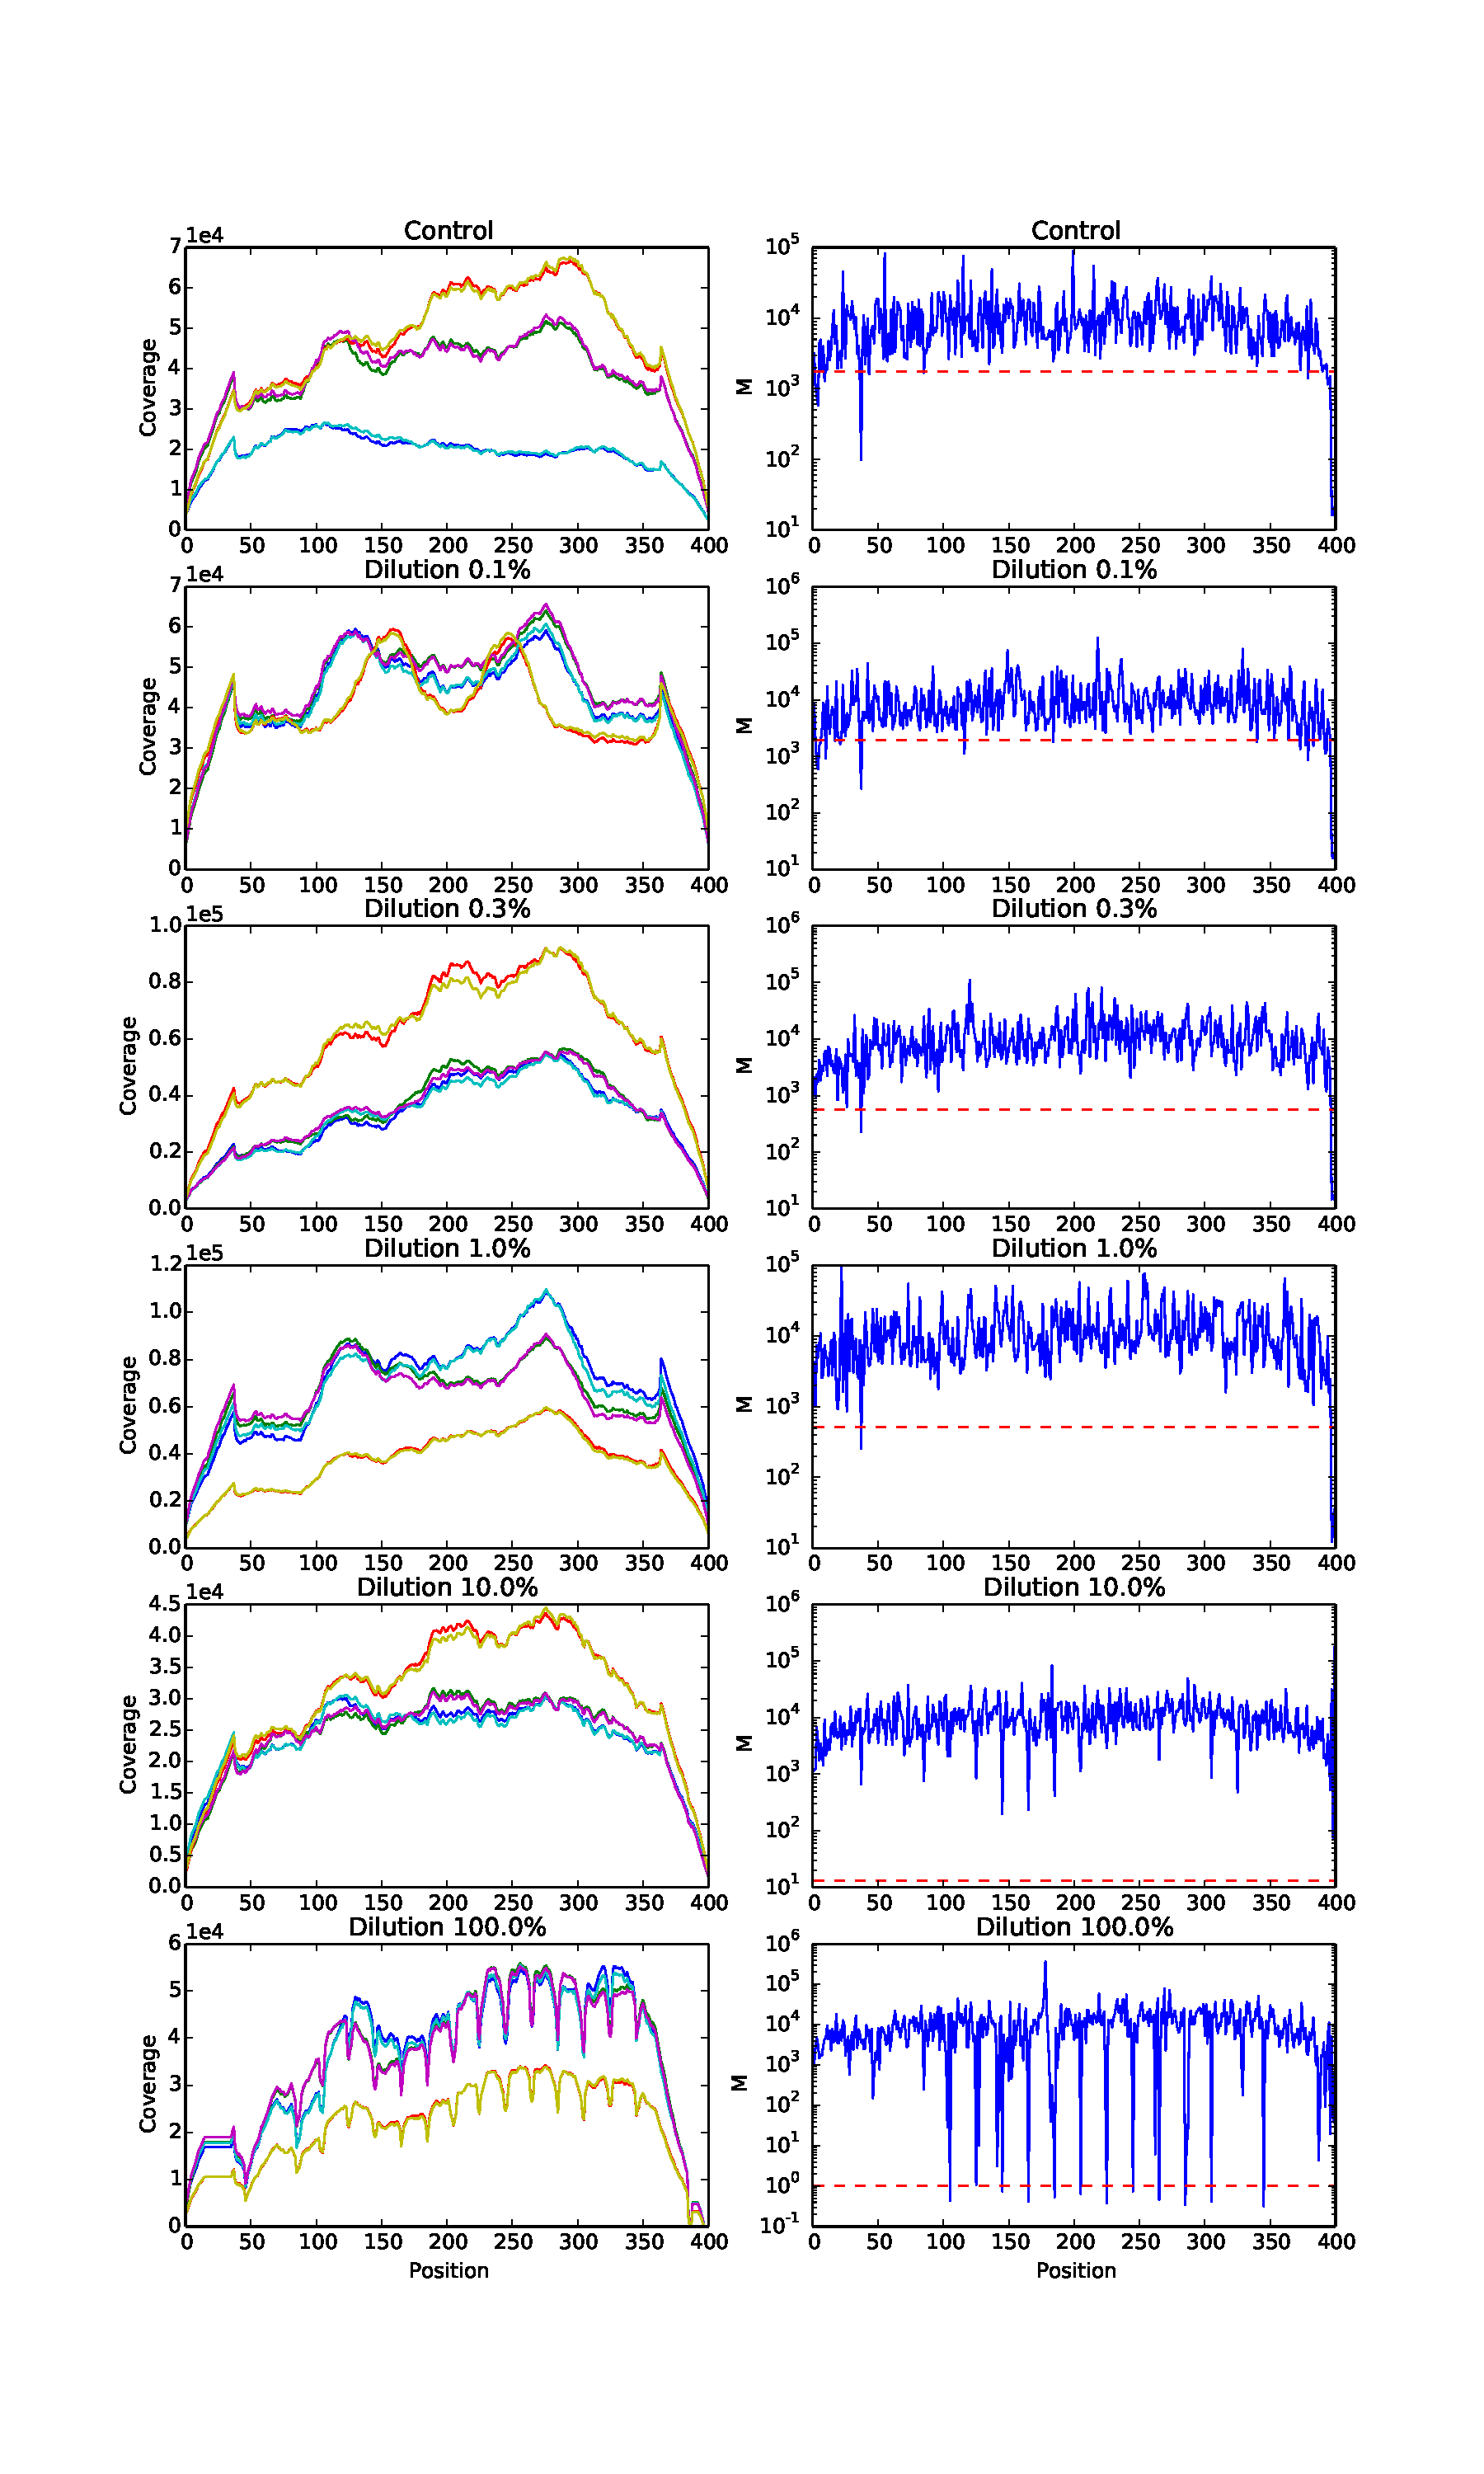
\includegraphics[width=90mm]{figs/M_jeffrey.pdf}
\caption{Key parameters for RVD3 model with Jeffreys prior on synthetic DNA data sets.}
\label{fig:M_jeffrey}
\end{center}
\end{figure}

\begin{figure*}[!tbp]
\begin{center}
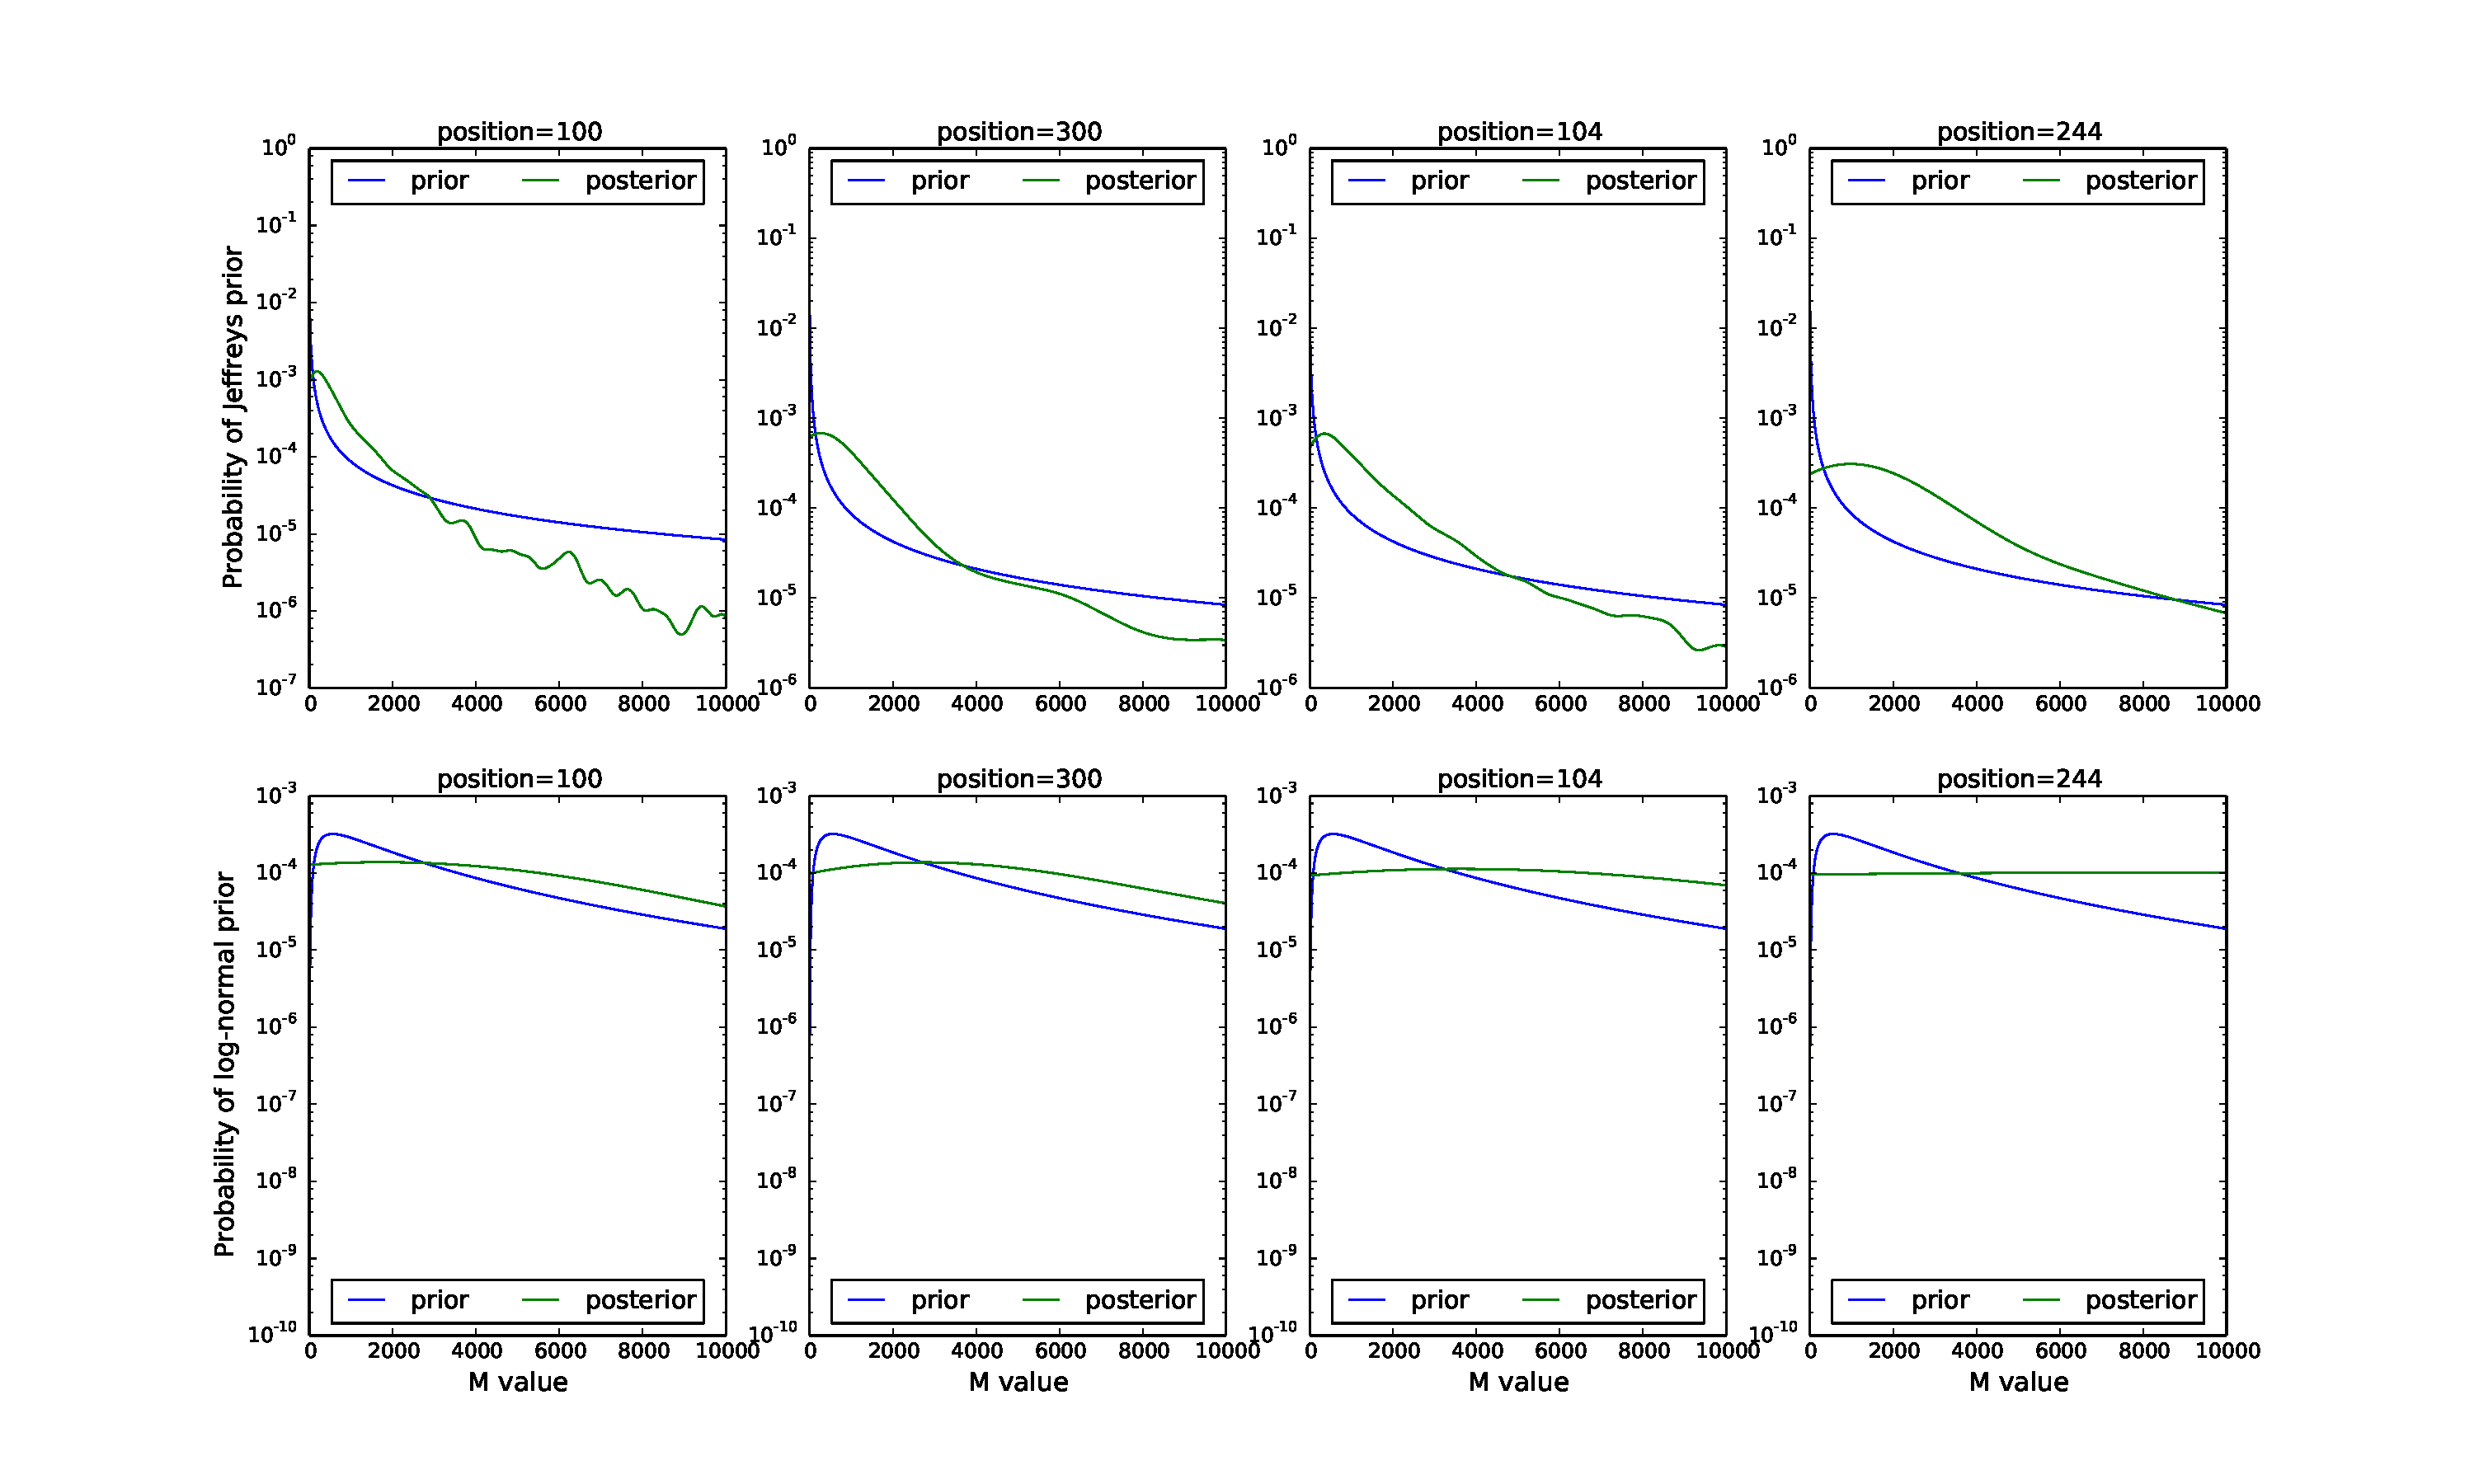
\includegraphics[width=190mm]{figs/post_prior_dilu_10.pdf}
\caption{Distribution of priors and posteriors when dilution is 10\%}
\label{fig:dilu_10}
\end{center}
\end{figure*}


Statistically, We analyzed the posteriors and priors for Jeffreys prior and log-normal prior. Figure~\ref{fig:dilu_10} shows the probability distribution over different M values when dilution is 10\% at $100\times$ read depth rate. The positions are chosen in the middle of the base length- position 104 and 244 are mutant, and position 100 and 300 are non-mutant. From the posterior probability distributions are estimated by Gaussian Kernel Density \citep{silverman1986density}. From the figure non-mutant positions display normal and stable without a peak nor a strange shape. The Jeffreys' prior shows more information than the lognormal prior (flat) from the posterior curve. From the prior distribution, it shows our model wants to search for a small value for M.

%%%%%%%%%%%%%%%%%%%%%%%%%%%%%
% Results of priors on synthetic data
%%%%%%%%%%%%%%%%%%%%%%%%%%%%%
\subsection{Results of priors on synthetic data}
\subsubsection{Performance with read depth}

\begin{figure}[htbp]
\begin{center}
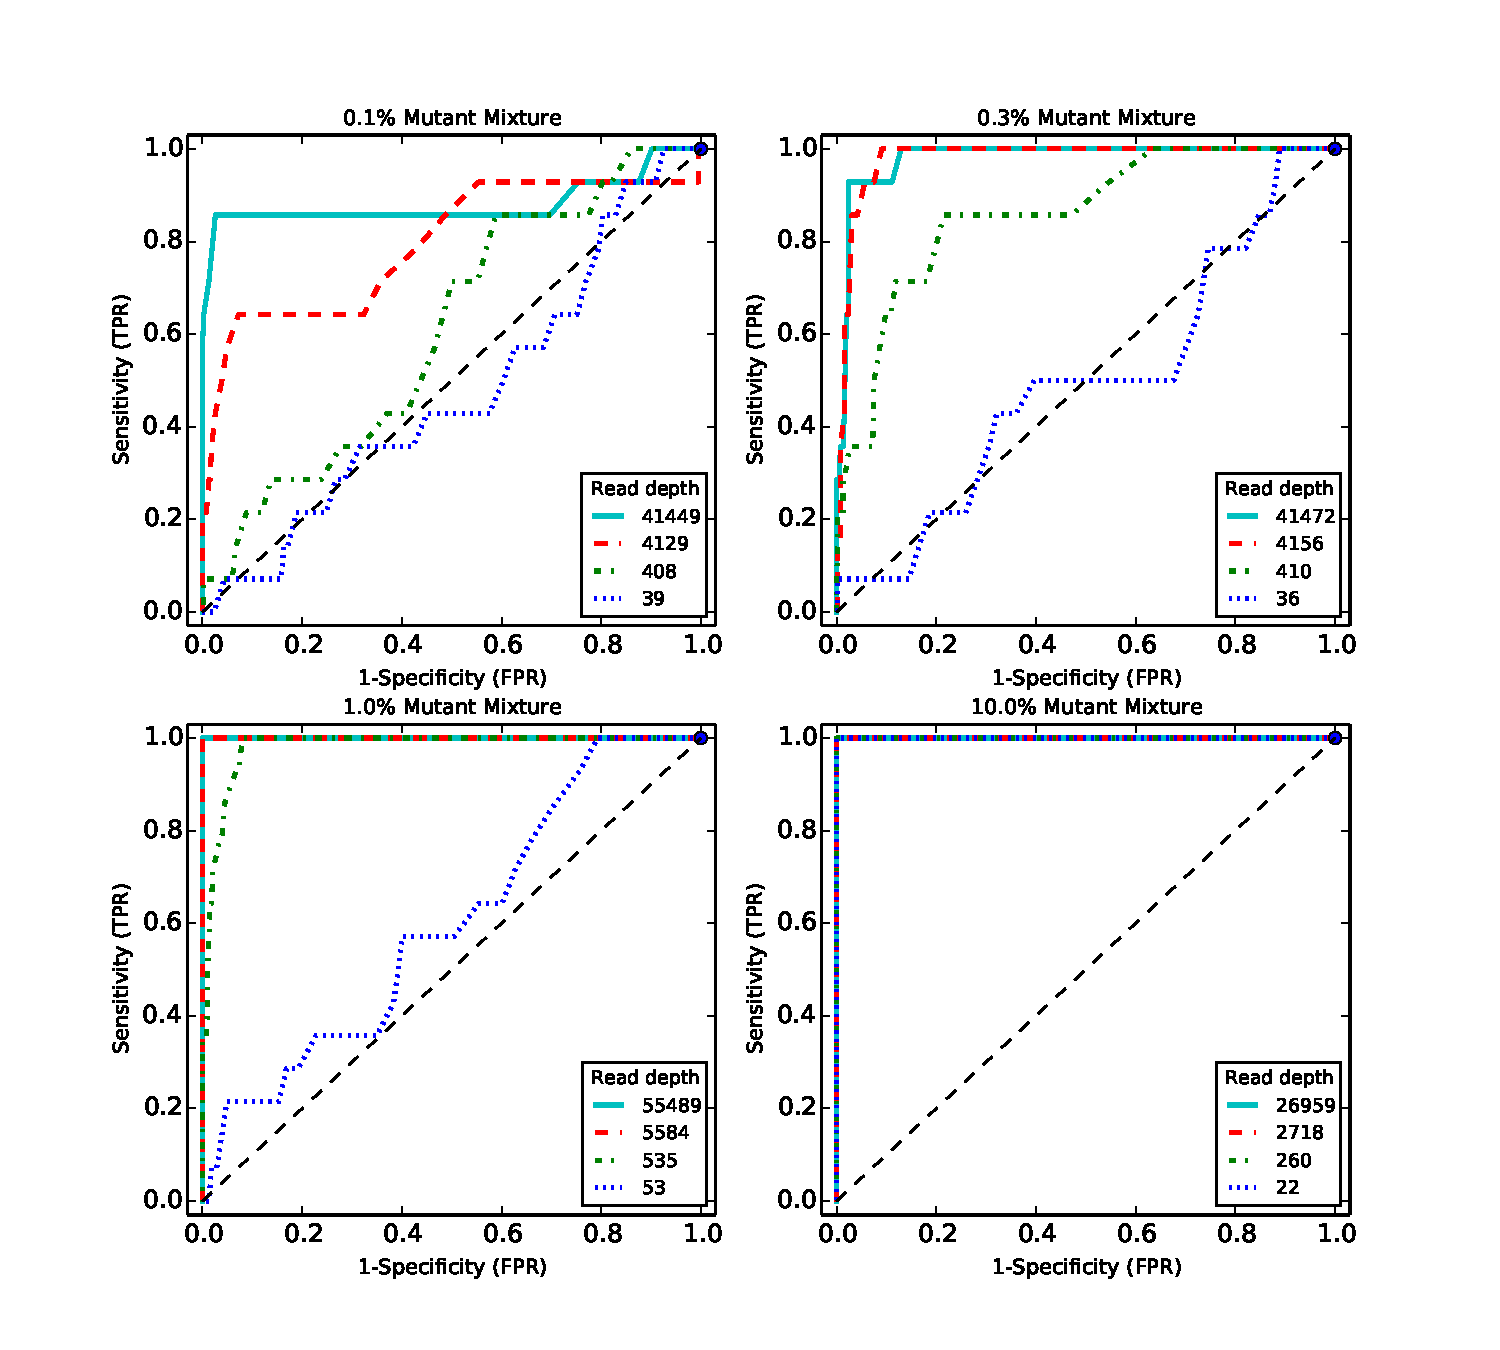
\includegraphics[width=90mm]{figs/ROC_without_chi2_jeffrey.pdf}
\caption{ROC curve for variants detection performance by Jeffreys prior.}
\label{fig:ROC_jeffrey}
\end{center}
\end{figure}

\begin{figure}[htbp]
\begin{center}
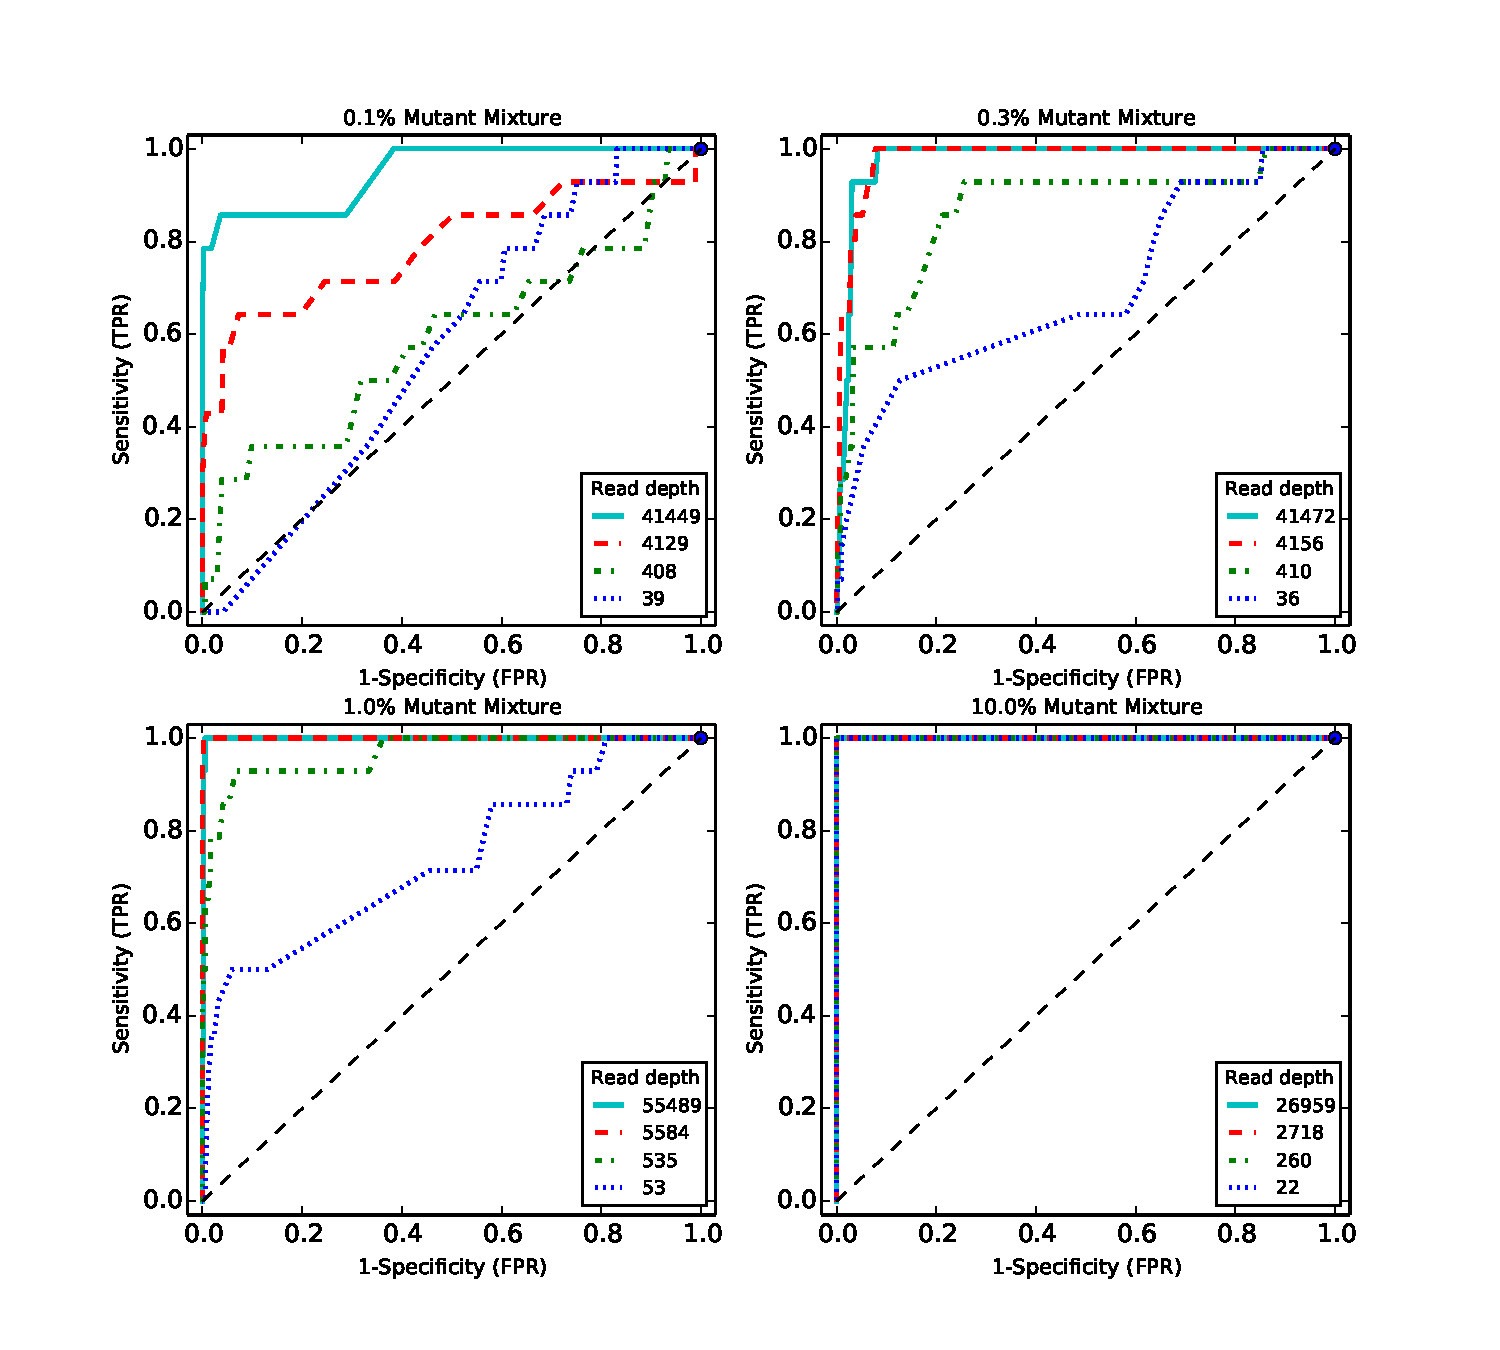
\includegraphics[width=90mm]{figs/ROC_without_chi2_lognormal.pdf}
\caption{ROC curve for variants detection performance by log-normal prior.}
\label{fig:ROC_lognormal}
\end{center}
\end{figure}


To evaluate the performance of RVD3 model with priors, we generated receiver-operating characteristic curves (ROCs) for median read depth and minor allele frequencies (MAFs). Here the Bayesian test is used without the $\chi^2$ test. Figure~\ref{fig:ROC_jeffrey} and Figure~\ref{fig:ROC_lognormal} shows ROC curves with a fixed $\alpha=0.05$. The performance improves when the read depth goes up. (ROC shows that the model with priors performs better than improper prior situation especially on the small read depth). Noticed at the lowest depth (22) with 10.0\% mutant mixture, the sensitivity and specificity value are 1 and much better than the model with improper priors for $M_j$, which definitely demonstrates the advantage of priors.

\subsubsection{Sensitivity/Specificity/FDR}

Figure~\ref{fig:SS} shows that the sensitivity and specificity of the RVD3 of different priors compared with the model with improper priors. Log-normal prior shows a higher sensitivity and specificity value than the Jeffreys prior.
Figure~\ref{fid:FDR} shows the false discovery rate of the RVD3 with different priors. Jeffreys prior shows a smaller false discovery rate and higher accuracy than others. It is obvious no matter Jeffreys or log-normal, the variant detection performance acquires lower FDR than the model with improper priors. Based on the various advantages for Jeffreys and log-normal prior, RVD3 can afford a more appropriate choice for the precision parameter. Here we chose Jeffreys prior model because it's a non-information prior, and more attention should be paid to false discovery rate and accuracy for variants calling research, compared with the clinical experiment or diagnosis which cares more on true positive rate and true negative rate.

\begin{figure}[htbp]
\begin{center}
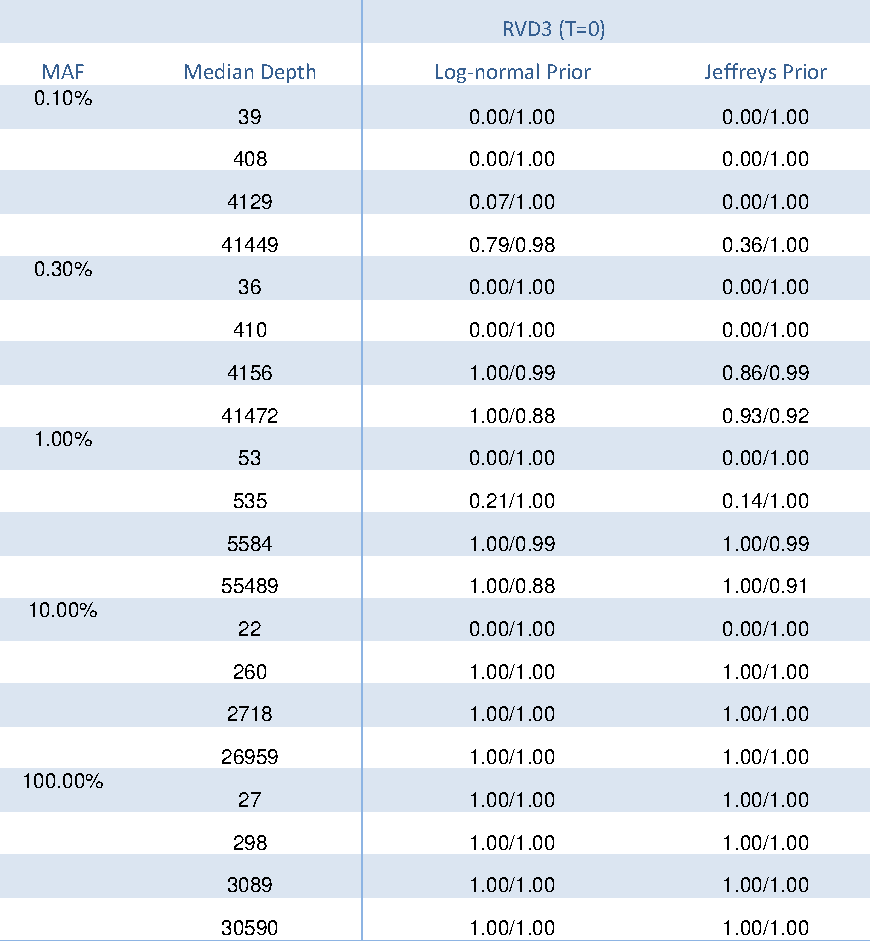
\includegraphics[width=80mm]{tables/Sen_Speci.pdf}
\caption{Sensitivity/Specificity comparison of RVD3 with different priors.}
\label{fig:SS}
\end{center}
\end{figure}


\begin{figure}[htbp]
\begin{center}
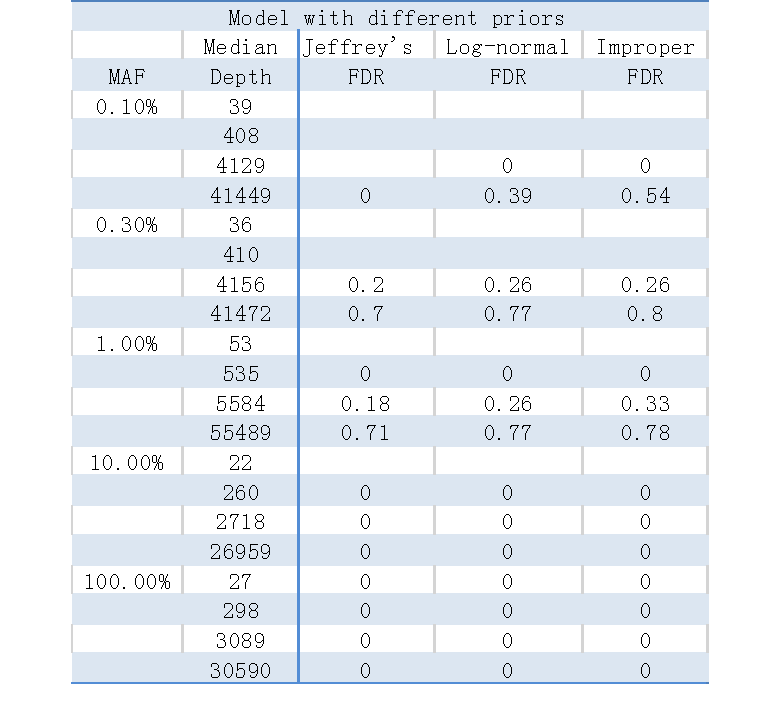
\includegraphics[width=80mm]{tables/FDR.pdf}
\caption{False Discovery Rate comparison of RVD3 with different priors.}
\label{fig:FDR}
\end{center}
\end{figure}

%%%%%%%%%%%%%%%%%%%%%%%%%%%%%%
% Results of Jeffreys prior on yeast data
%%%%%%%%%%%%%%%%%%%%%%%%%%%%%%
\subsection{Results of Jeffreys prior on yeast data}

We demonstrated our RVD3 model with Jeffreys prior on yeast data to identify the variants \citep{Flaherty:2011ja}.



\section{Discussion}
analysis of the tradeoff between experimental precision and sequencing depth to achieve ultrasensitive variant detection.


%%%%%%%%%%%%%%%%%%%%%%%%%%%%%%%%%%%%%%%%%%%%%%%%%%%%%%%%%%%%%%%%%%%%%%%%%%%%%%%%%%%%%
%
%     please remove the " % " symbol from \centerline{\includegraphics{fig01.eps}}
%     as it may ignore the figures.
%
%%%%%%%%%%%%%%%%%%%%%%%%%%%%%%%%%%%%%%%%%%%%%%%%%%%%%%%%%%%%%%%%%%%%%%%%%%%%%%%%%%%%%%


\section{Conclusion}



\begin{enumerate}
\item this is item, use enumerate
\item this is item, use enumerate
\item this is item, use enumerate
\end{enumerate}


\section*{Acknowledgement}
Text Text

\paragraph{Funding\textcolon} Text Text  Text Text.

\bibliographystyle{natbib}
%\bibliographystyle{achemnat}
%\bibliographystyle{plainnat}
%\bibliographystyle{abbrv}
%\bibliographystyle{bioinformatics}
%\bibliographystyle{plain}

\bibliography{bioinfo}


\appendix

%%%%%%%%%%%%%%%%%%%
% Appendix A: Parameter Initialization
%%%%%%%%%%%%%%%%%%%
\section{Parameter Initialization}\label{sec:appendix_mom}
Since $r_{ji} \thicksim \text{Binomial}(n_{ji}, \theta_{ji})$, the first population moment is  $E[r_{ji}] = \theta_{ji} n_{ji}$ and the first sample moment is simply $m_1 = r_{ji}$. Therefore the MoM estimator is
\begin{equation}
	\tilde{\theta}_{ji} = \frac{r_{ji}} {n_{ji}}
\end{equation}

We take the MoM estimate, $\tilde{\theta}_{ji}$, as data for the next conditional distribution in the hierarchical model. The distribution is $\theta_{ji} \thicksim \text{Beta}(\mu_jM_j, (1-\mu_j)M_j)$. The first and second population moments are
\begin{eqnarray}
	E[\theta_{ji}] =& \mu_j,\\
	\text{Var}[\theta_{ji}] =& \frac{\mu_j(1-\mu_j)} { M_j + 1 }.
\end{eqnarray}
The first and second sample moments are $m_1 = \frac{1}{N}\sum_{i=1}^N \theta_{ji}$ and $m_2 = \frac{1}{N}\sum_{i=1}^N \theta_{ji}^2$. Setting the population moments equal to the sample moments and solving for $\mu_j$ and $M_j$ gives
\begin{eqnarray}
	\tilde{\mu}_j =& \frac{1}{N} \sum_{i=1}^N \theta_{ji}, \\
	\tilde{M_j} =& \frac{ \tilde{\mu}_j (1 - \tilde{\mu}_j ) } { \frac{1}{N} \sum_{i=1}^N \theta_{ji}^2 } -1.
\end{eqnarray}

Following the same procedure for the parameters of $\mu_j \thicksim \text{Beta}(\mu_0, M_0)$ gives the following MoM estimates
\begin{eqnarray}
	\tilde{\mu}_0 =& \frac{1}{J} \sum_{j=1}^J \mu_j \\
	\tilde{M}_0 =& \frac{ \tilde{\mu}_0 (1 - \tilde{\mu}_0 ) } {\frac{1}{J} \sum_{j=1}^J \mu_j^2 } -1.
\end{eqnarray}

%%%%%%%%%%%%%%%%%%%
% Appendix B: Inference of Jeffreys prior
%%%%%%%%%%%%%%%%%%%
\section{Inference of Jeffreys prior}\label{sec:appendix_Jeffreys}
We assume there is only one replicate,

\begin{equation}\label{eqn:Betapdf}
p\left({\theta }_{j} \right)= \frac{\Gamma \left({M}_{j} \right)}{\Gamma \left({\mu }_{j} {M}_{j}\right)\Gamma \left(( 1-{\mu }_{j}){M}_{j}\right)} {{\theta}_{j}}^{{\mu}_{j}{M}_{j}-1}{\left(1-\theta\right)_{j}}^{\left(1-{\mu}_{j}\right){M}_{j}-1}
\end{equation}

\begin{equation}\label{equ:JefferyInference1}
\begin{split}
\log p\left(\theta_{j}|\mu_{j},M_{j}\right)& =\log \Gamma \left(M_{j}\right)-\log \Gamma\left(\mu_{j},M_{j}\right)- \log \Gamma\left(1-\mu_{j},M_{j}\right)\\
& + (\mu_{j}M_{j}-1)\log\theta_{j} + ((1-\,u_{j})M_{j}-1)\log(1-\theta_{j})\
\end{split}
\end{equation}

\begin{equation}
\frac{\delta\log p(\theta_{j})}{\delta M_{j}} = \Psi(M_{j}) - \Psi(\mu_{j} M_{j})\mu_{j} - \Psi((1-\mu_{j})M_{j})(1-\mu_{j}) +\mu_{j}\log\theta_{j} + (1-\mu_{j})\log(1-\theta_{j})
\end{equation}

\begin{equation}
\frac{\delta^{2}\log p(\theta_{j})}{\delta M_{j}^{2}}  = \Psi_{1}(M_{j}) - \Psi_{1}(\mu_{j} M_{j})\mu_{j}^{2} - \Psi_{1}((1-\mu_{j})M_{j})(1-\mu_{j})^{2}
\end{equation}

Now we have the Jeffreys' prior for $M_{j}$:

\begin{equation}
[-\left(\Psi_{1}(M_{j}) - \Psi_{1}(\mu_{j} M_{j})\mu_{j}^{2} - \Psi_{1}((1-\mu_{j})M_{j}){(1-\mu_{j})^{2}}\right)]^{\frac{1}{2}}
\end{equation}

%%%%%%%%%%%%%%%%%%%
% Appendix C: Key parameters for RVD3 model with log-normal prior
%%%%%%%%%%%%%%%%%%%

\section{Key parameters for RVD3 model with log-normal prior}\label{sec:appendix_parameters}
Key parameters of the RVD3 with log-normal prior is ploted in Figure~\ref{fig:M_lognormal}.

\begin{figure}[htbp]
\begin{center}
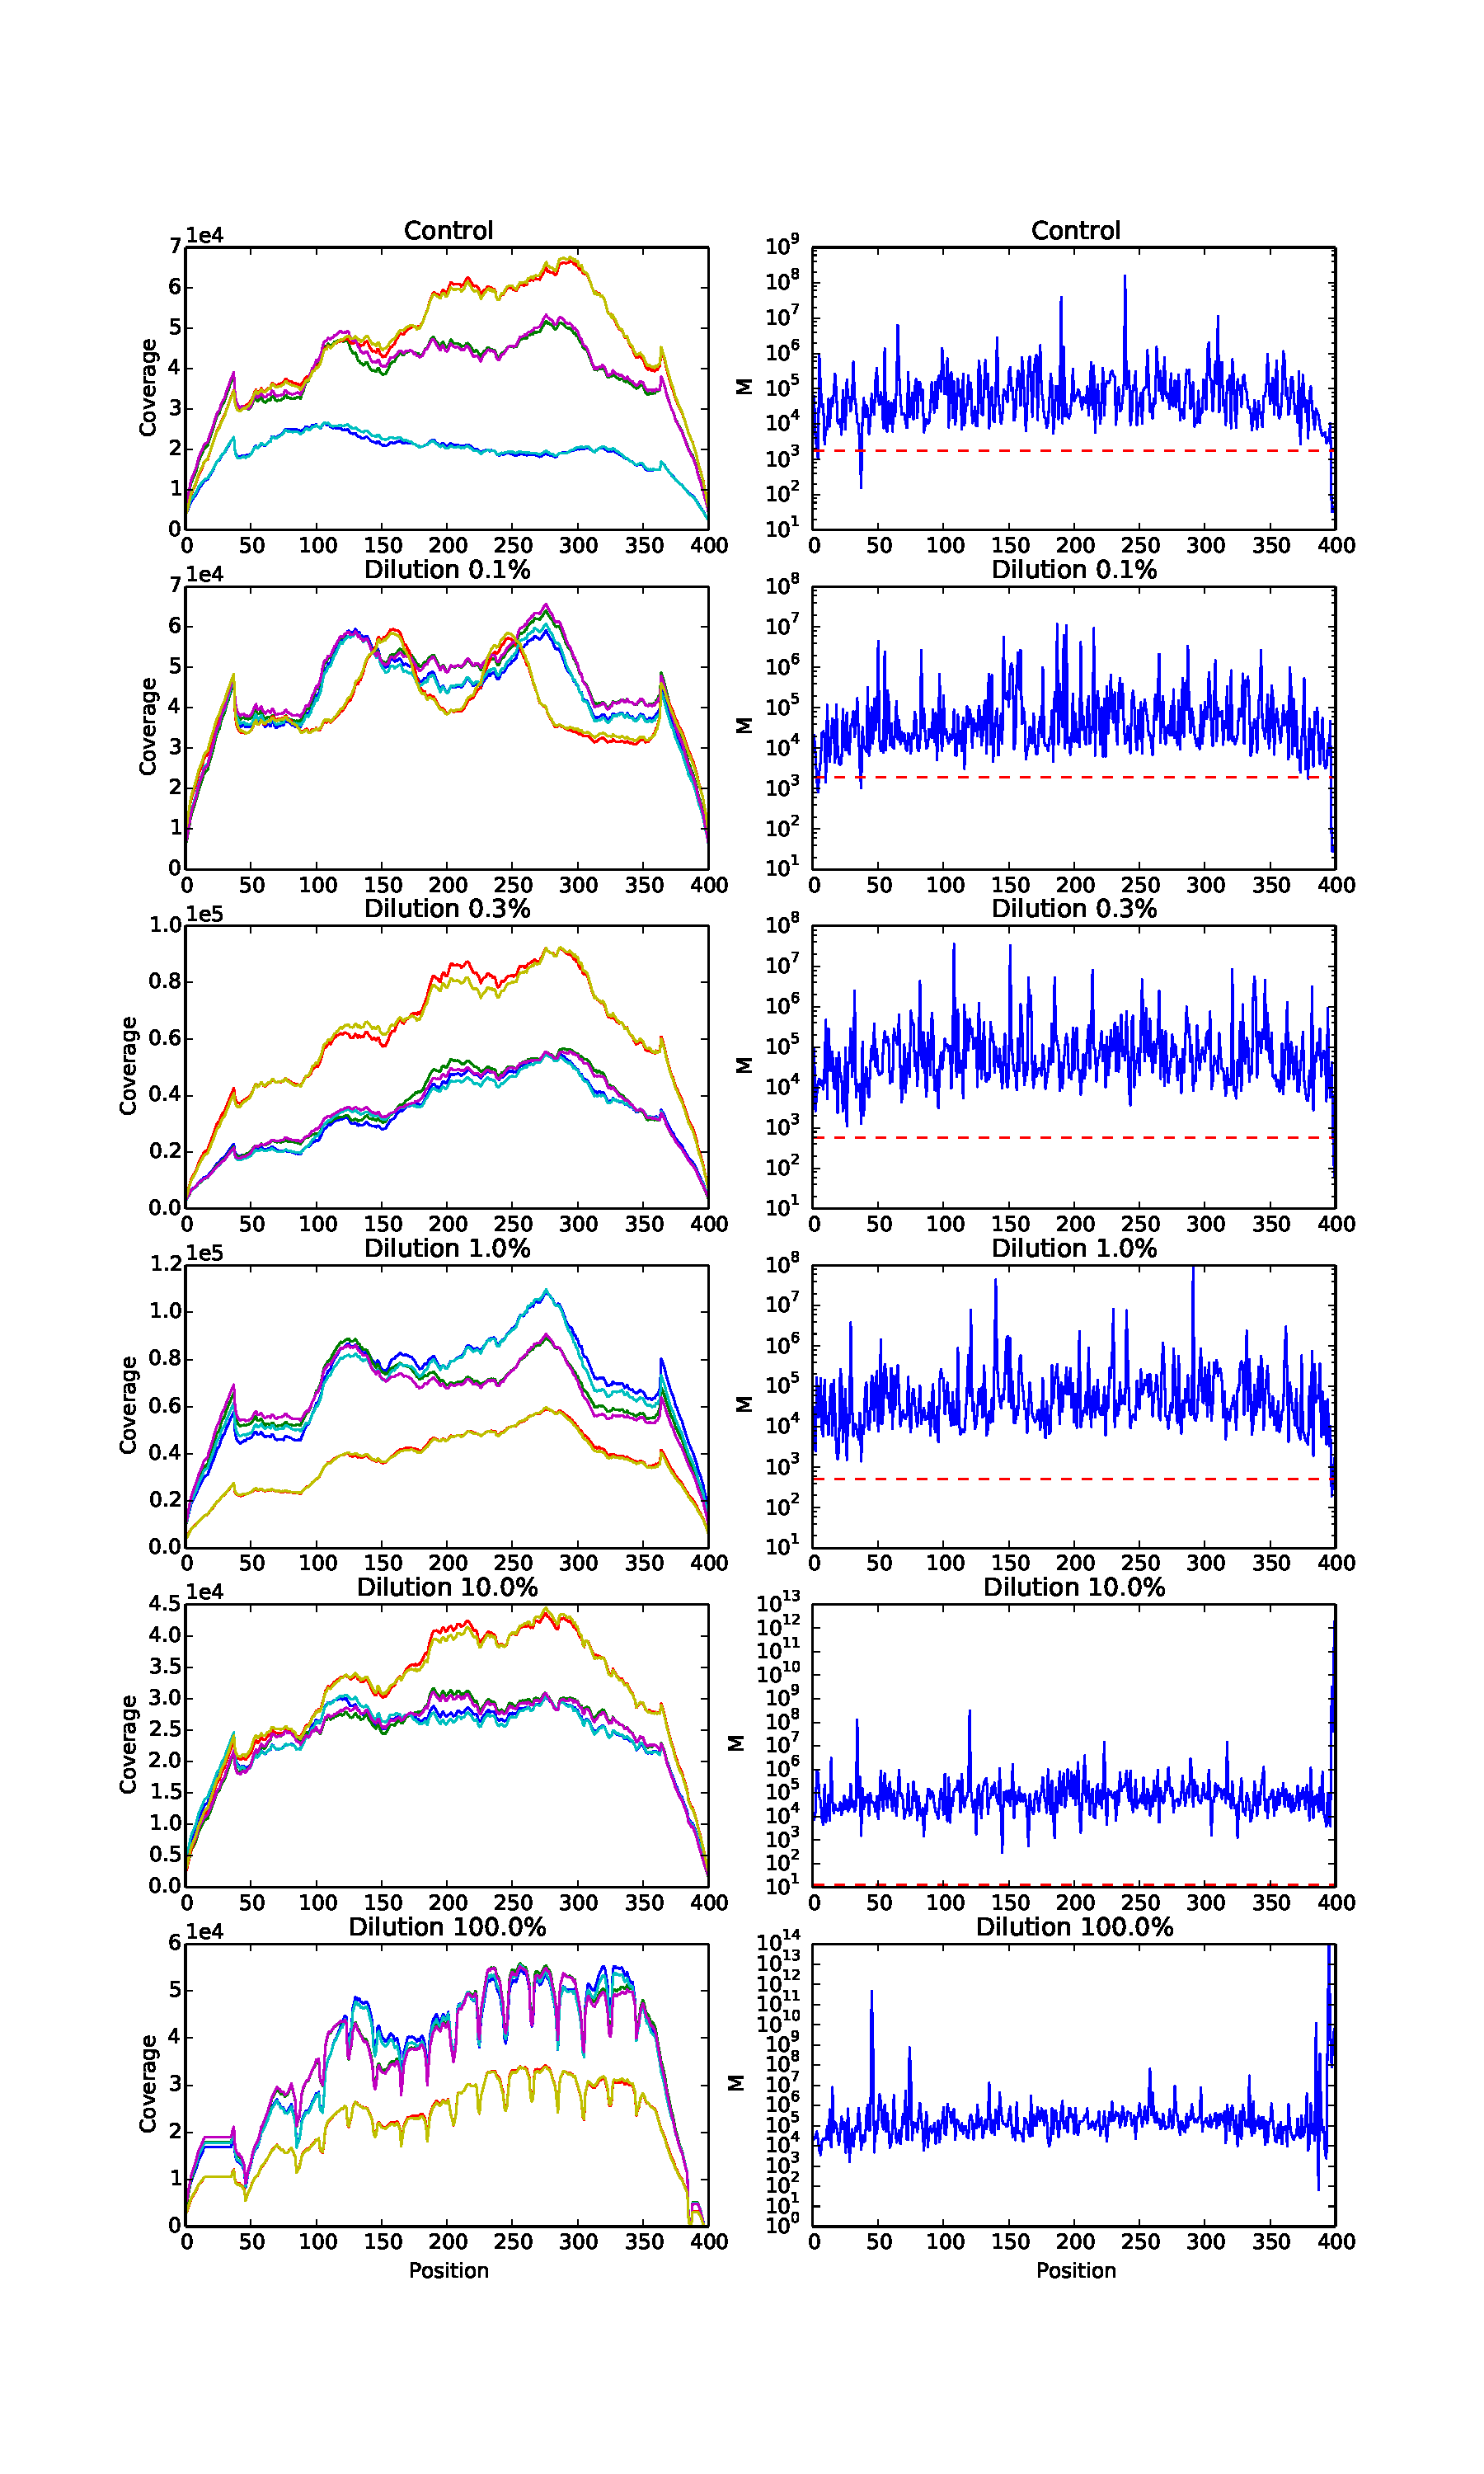
\includegraphics[width=90mm]{figs/M_lognormal.pdf}
\caption{Key parameters for RVD3 model with log-normal prior for synthetic DNA data sets.}
\label{fig:M_lognormal}
\end{center}
\end{figure}


\end{document}
